\uuid{xaHb}
\exo7id{2850}
\titre{exo7 2850}
\auteur{burnol}
\organisation{exo7}
\datecreate{2009-12-15}
\isIndication{false}
\isCorrection{false}
\chapitre{Théorème des résidus}
\sousChapitre{Théorème des résidus}
\module{Analyse complexe}
\niveau{L3}
\difficulte{}

\contenu{
\texte{
Soit $\gamma$ le contour, parcouru dans le sens direct, dessiné ci-contre. 
$$\centerline{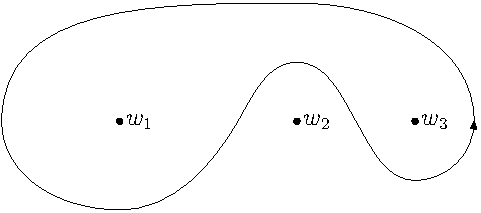
\includegraphics{../images/pdf/xaHb-1.pdf}}$$

Déterminer (avec justification) en fonction de $w_1$, $w_2$, $w_3$ les intégrales suivantes:
\begin{align*}
A &= \int_\gamma \frac{dz}{(z-w_1)(z-w_2)(z-w_3)}\\
B &= \int_\gamma \sin(z) dz\\
C &= \int_\gamma \frac{dz}{(z-w_1)^2(z-w_3)}
\end{align*}
}
}
